\documentclass[11pt,preprint, authoryear]{elsarticle}

\usepackage{lmodern}
%%%% My spacing
\usepackage{setspace}
\setstretch{1.2}
\DeclareMathSizes{12}{14}{10}{10}

% Wrap around which gives all figures included the [H] command, or places it "here". This can be tedious to code in Rmarkdown.
\usepackage{float}
\let\origfigure\figure
\let\endorigfigure\endfigure
\renewenvironment{figure}[1][2] {
    \expandafter\origfigure\expandafter[H]
} {
    \endorigfigure
}

\let\origtable\table
\let\endorigtable\endtable
\renewenvironment{table}[1][2] {
    \expandafter\origtable\expandafter[H]
} {
    \endorigtable
}


\usepackage{ifxetex,ifluatex}
\usepackage{fixltx2e} % provides \textsubscript
\ifnum 0\ifxetex 1\fi\ifluatex 1\fi=0 % if pdftex
  \usepackage[T1]{fontenc}
  \usepackage[utf8]{inputenc}
\else % if luatex or xelatex
  \ifxetex
    \usepackage{mathspec}
    \usepackage{xltxtra,xunicode}
  \else
    \usepackage{fontspec}
  \fi
  \defaultfontfeatures{Mapping=tex-text,Scale=MatchLowercase}
  \newcommand{\euro}{€}
\fi

\usepackage{amssymb, amsmath, amsthm, amsfonts}

\def\bibsection{\section*{References}} %%% Make "References" appear before bibliography


\usepackage[round]{natbib}

\usepackage{longtable}
\usepackage[margin=2.3cm,bottom=2cm,top=2.5cm, includefoot]{geometry}
\usepackage{fancyhdr}
\usepackage[bottom, hang, flushmargin]{footmisc}
\usepackage{graphicx}
\numberwithin{equation}{section}
\numberwithin{figure}{section}
\numberwithin{table}{section}
\setlength{\parindent}{0cm}
\setlength{\parskip}{1.3ex plus 0.5ex minus 0.3ex}
\usepackage{textcomp}
\renewcommand{\headrulewidth}{0.2pt}
\renewcommand{\footrulewidth}{0.3pt}

\usepackage{array}
\newcolumntype{x}[1]{>{\centering\arraybackslash\hspace{0pt}}p{#1}}

%%%%  Remove the "preprint submitted to" part. Don't worry about this either, it just looks better without it:
\makeatletter
\def\ps@pprintTitle{%
  \let\@oddhead\@empty
  \let\@evenhead\@empty
  \let\@oddfoot\@empty
  \let\@evenfoot\@oddfoot
}
\makeatother

 \def\tightlist{} % This allows for subbullets!

\usepackage{hyperref}
\hypersetup{breaklinks=true,
            bookmarks=true,
            colorlinks=true,
            citecolor=blue,
            urlcolor=blue,
            linkcolor=blue,
            pdfborder={0 0 0}}


% The following packages allow huxtable to work:
\usepackage{siunitx}
\usepackage{multirow}
\usepackage{hhline}
\usepackage{calc}
\usepackage{tabularx}
\usepackage{booktabs}
\usepackage{caption}


\newenvironment{columns}[1][]{}{}

\newenvironment{column}[1]{\begin{minipage}{#1}\ignorespaces}{%
\end{minipage}
\ifhmode\unskip\fi
\aftergroup\useignorespacesandallpars}

\def\useignorespacesandallpars#1\ignorespaces\fi{%
#1\fi\ignorespacesandallpars}

\makeatletter
\def\ignorespacesandallpars{%
  \@ifnextchar\par
    {\expandafter\ignorespacesandallpars\@gobble}%
    {}%
}
\makeatother

\newlength{\cslhangindent}
\setlength{\cslhangindent}{1.5em}
\newenvironment{CSLReferences}%
  {\setlength{\parindent}{0pt}%
  \everypar{\setlength{\hangindent}{\cslhangindent}}\ignorespaces}%
  {\par}


\urlstyle{same}  % don't use monospace font for urls
\setlength{\parindent}{0pt}
\setlength{\parskip}{6pt plus 2pt minus 1pt}
\setlength{\emergencystretch}{3em}  % prevent overfull lines
\setcounter{secnumdepth}{5}

%%% Use protect on footnotes to avoid problems with footnotes in titles
\let\rmarkdownfootnote\footnote%
\def\footnote{\protect\rmarkdownfootnote}
\IfFileExists{upquote.sty}{\usepackage{upquote}}{}

%%% Include extra packages specified by user

%%% Hard setting column skips for reports - this ensures greater consistency and control over the length settings in the document.
%% page layout
%% paragraphs
\setlength{\baselineskip}{12pt plus 0pt minus 0pt}
\setlength{\parskip}{12pt plus 0pt minus 0pt}
\setlength{\parindent}{0pt plus 0pt minus 0pt}
%% floats
\setlength{\floatsep}{12pt plus 0 pt minus 0pt}
\setlength{\textfloatsep}{20pt plus 0pt minus 0pt}
\setlength{\intextsep}{14pt plus 0pt minus 0pt}
\setlength{\dbltextfloatsep}{20pt plus 0pt minus 0pt}
\setlength{\dblfloatsep}{14pt plus 0pt minus 0pt}
%% maths
\setlength{\abovedisplayskip}{12pt plus 0pt minus 0pt}
\setlength{\belowdisplayskip}{12pt plus 0pt minus 0pt}
%% lists
\setlength{\topsep}{10pt plus 0pt minus 0pt}
\setlength{\partopsep}{3pt plus 0pt minus 0pt}
\setlength{\itemsep}{5pt plus 0pt minus 0pt}
\setlength{\labelsep}{8mm plus 0mm minus 0mm}
\setlength{\parsep}{\the\parskip}
\setlength{\listparindent}{\the\parindent}
%% verbatim
\setlength{\fboxsep}{5pt plus 0pt minus 0pt}



\begin{document}



\begin{frontmatter}  %

\title{Sustainability in the Political Economy}

% Set to FALSE if wanting to remove title (for submission)




\author[Add1]{Harriet Catherine Laing}
\ead{nfkatzke@gmail.com}





\address[Add1]{University of Stellenbosch, South Africa}

\cortext[cor]{Corresponding author: Harriet Catherine Laing}

\begin{abstract}
\small{
Abstract to be written here. The abstract should not be too long and
should provide the reader with a good understanding what you are writing
about. Academic papers are not like novels where you keep the reader in
suspense. To be effective in getting others to read your paper, be as
open and concise about your findings here as possible. Ideally, upon
reading your abstract, the reader should feel he / she must read your
paper in entirety.
}
\end{abstract}

\vspace{1cm}


\begin{keyword}
\footnotesize{
Multivariate GARCH \sep Kalman Filter \sep Copula \\
\vspace{0.3cm}
}
\end{keyword}



\vspace{0.5cm}

\end{frontmatter}



%________________________
% Header and Footers
%%%%%%%%%%%%%%%%%%%%%%%%%%%%%%%%%
\pagestyle{fancy}
\chead{}
\rhead{}
\lfoot{}
\rfoot{\footnotesize Page \thepage}
\lhead{}
%\rfoot{\footnotesize Page \thepage } % "e.g. Page 2"
\cfoot{}

%\setlength\headheight{30pt}
%%%%%%%%%%%%%%%%%%%%%%%%%%%%%%%%%
%________________________

\headsep 35pt % So that header does not go over title




\hypertarget{introduction}{%
\section{\texorpdfstring{Introduction
\label{Introduction}}{Introduction }}\label{introduction}}

(approx. 800)

The primary objective of this research assignment is to model how
interactions in the political economy inhibit the advancement of
environmental policies. Ultimately, we wish to understand how the
frictions and dominance of certain countries in the global area impacts
global environmental policy. For example, the US is a relatively smaller
country with a large dominant role in the global arena that has a
greater voting weight, compared to larger countries geographically with
less dominance politically. This results in sub-optimal outcomes such as
dominant countries contributing to pollution in larger countries that
are geographically positioned in relatively more vulnerable positions.
The model we set up first considers the simplest case of a two-period
optimisation problem. There is a world with abundant resources, where
consumers believe that they can consume a lot today and tomorrow, and
information about the state of the world is aggregated perfectly. As we
continue to model this problem, frictions are added. For example, the
state of the world may not be aggregated correctly to the voters. For
our model, the focus is how the political system works when there is the
issue of environmental degradation. Accordingly, the literature on both
sides of the sustainability of the political economy is considered.
Namely, the literature on exhaustible resources (including the optimal
depletion thereof and the cake-eating optimisation problem) and the
political economy (including the aggregation of political information
and strategic voting).

The first specification of the state of the world will be modeled within
a global economy in which there is only one population of voters and
information is aggregated imperfectly. The second specification of the
model will introduce the two-country setting and how adjustments to the
bias of voter signals and the relative size of the countries may affect
each country's citizens' voting decisions. Thereafter, the two
specifications will be compared to each other to determine how
co-operation between countries with regards to environmental policies
may be disadvantageous for consumption and may make the probability of a
crisis more likely.

\hypertarget{literature-review}{%
\section{Literature review}\label{literature-review}}

(approx. 2000)

Pindyck (1978) models two optimal paths for using non-renewable
resources depending on the initial resource endowment and the different
marginal costs of extraction. If the initial reserve is large, then this
will cause extraction costs to be low and thereby price will slowly rise
over time. On the other hand, if the initial reserve has been depleted
and is small, both the price and the extraction costs will be high. As
reserves decline, the production cost for using resources increases and
potential profits reduces. Accordingly, as marginal costs increase for
extraction, producers will begin to conserve non-renewable resources
because the marginal benefit thereof is smaller. Therefore, for
non-renewable resources with a fixed reserve its time horizon can be
increased with economic incentives such as profit opportunities that
increase exploratory activity; ``potential reserves'' are unlimited.
However, the model does not include the situation in which the
non-renewable quantities are uncertain.

Kemp (1976) was the first to consider the cake-eating optimisation
problem for an exhaustible resource of an unknown size and the idea has
since been developed in the literature. Loury (1978) investigates the
problem of optimal planning when faced with two issues in this regard;
(i) the possibility of exhaustion of the resource, and (ii) learning
about the distribution of reserves over time through exploration and
extraction activities. Under certainty when a resource's reserve is
known, the possibility of exhaustion occurs only asymptotically.
However, when the resource base is of unknown size, the date on which it
will have been completely exploited is also a random variable. The
choice of the rate of consumption is necessarily affected by the impact
of the consumption rate on the probability of `crisis', or likelihood of
reaching the tipping point. Therefore, this paper demonstrates that the
possibility of premature exhaustion alters the requirements of an
optimal consumption path. The model used in the paper includes the date
upon which the resource is exhausted as a choice variable and specifies
some minimal level of resource consumption that is necessary to sustain
an economy. ``Set the objective function as the maximisation of the
expected value of the integral of discounted utility. Employ dynamic
programming techniques to deduce some comparative static results'' The
uncertain reserve is a random variable that is drawn from a cumulative
density function.

Kumar (2005) reconsiders Kemp's use of an infinite planning horizon by
instead using a hazard function which is defined as the probability of
reaching the climate tipping point. The paper argues that `cake-eating
under uncertainty' has two main aspects: (i) optimal planning horizon
and (ii) the characterisation of optimal program. The former aspect of
the (i) optimal planning horizon can be assumed to extend far enough
into the future to allow for the resource to be fully exhausted at some
point. By employing a hazard function to model the problem, this
planning horizon over which consumption of the exhaustible resource is
positive has been found to be either finite or infinite. The findings of
Kumar (2005) are that if an uncertain resource stock is finite and the
optimal planning horizon is finite, hazard rates increase in unbounded
fashion, and marginal utility of extraction and consumption at zero is
finite. However, if an uncertain resource stock size is unbounded, the
planning horizon is infinite. Thus, the optimal rate of extraction and
consumption over time generally moves monotonically in the opposite
direction to the hazard rate.

Adler \& Treich (2017) consider additional elements that are not
included in Kumar (2005) which are involved in the decision for optimal
climate policy. There are three dimensions of climate policy modelled:
(i) equity, (ii) time, and (iii) risk which each impact how risky
consumption is allocated intertemporally. The cake-eating problem for an
uncertain quantity of resources with a social planner allocating between
the current and future generation is modelled in terms of three
different social welfare functions. The first generation is given a
determinate amount of consumption, but the second generation is given
the risky remainder. The methodology used is a prioritarian social
welfare function (SWF) which is the sum of some increasing, concave
function of utility for the well-being of a generation. To find the
optimal consumption allocation, Adler \& Treich (2017) compare statics
analysis for the different functions.

Lemoine \& Traeger (2014) address the need to integrate policy with
possibility of climate tipping points into a benchmark integrated
assessment model'' to analyse the intertemporal trade-offs that
characterise climate policy decisions. Crossing the threshold shifts the
world permanently to a new altered system with different dynamics to
pre-threshold. The paper ``analytically demonstrated that tipping points
affect optimal policy via two channels: the differential welfare impact
(DWI) recognizes that today's policy choices affect welfare in the case
that a tipping point occurs, and the marginal hazard effect (MHE)
recognizes that today's policy choices affect the probability of
crossing the threshold.'' endogenises welfare and probability of tipping
point.

On the political economy side of the literature, Piketty (1999) provides
a short survey of recent contributions to the literature related to
political institutions as an information-aggregation mechanism.
Condorcet (1785) was the first to posit that political institutions have
a constructive role in efficiently aggregating information in a society.
His main contribution to the literature was termed the `Condorcet Jury
Theorem' which states that under free elections, the probability that
the the policy that is preferred by the majority will win by majority
vote tends to one as the number of individuals in the population tends
to infinity. This theorem posits democracy is an efficient
information-aggregation system if it is assumed that individuals are
homogenous in their initial prior beliefs about the state of the world,
each receives a signal drawn from the same conditional distribution and
that it is realistic that more than half of citizens are right/ more
than half of the time.

Many models of political economy include different stages to analyse how
voting impacts policies but vary according to how voters' derive utility
(Lohmann, 1994; Besley \& Coate, 1998; Razin, 2003; Buchholz \emph{et
al}, 2005). Lohmann (1994) investigated the impact of the information
aggregated by political action before a vote on whether votes cast are
more or less accurate, where accuracy is defined in terms of reflecting
voters' preferences. The paper models that each individual has a loss
function which dictates the loss if policy outcome is not what the
individual desired and the private cost if the individual engaged in
political action. The equilibrium point is where an individual's
political action strategy minimises her expected loss after the
political action stage, and thus an individual only engages in political
action if the cost of doing so is outweighed by the potential benefit of
achieving the political outcome she wants.

Razin (2003) models elections with two potential candidates in a
one-dimensional policy space. Voting behaviour is strategic as voters
are motivated by both the election and signalling implications of
voting. Razin (2003) assumes that voters are privately and imperfectly
informed about a common shock which impacts voters' preferences. Voters'
private signals are drawn independently from a distribution and are
conditional on the common shock. Razin (2003) also uses the policy gap
idea (how far is the actual policy outcome from the voter's
preference/ideal) in a utility function.

To analyse voter behaviour, Lohmann (1994) uses game theoretical best
responses at each stage are determined. For example, at the political
action stage, their best response is a function of the `type' of voter
they are and the individual preferences they have. Razin (2003) also
uses game theory with two stage process: First stage = common shock
dictated by nature and voters receive and observe independent and
private signals that are conditional upon this shock. Second stage =
voters cast ballots simultaneously for either candidate L or R (cannot
abstain from voting). Candidate with majority wins and chooses a policy
according to votes (assuming candidates are responsive).

Buchholz \emph{et al} (2005) investigates the policy outcome that may
arise from international environmental agreements when governments are
democratically elected by citizens. This paper considers two pertinent
themes, namely the case in which a voter may be incentivised to support
a political candidate who is less environmentally inclined than the
voter's own preferences and the case in which the elected candidate pays
no attention to environmental policies and thus international agreements
are rendered ineffective. The paper argues that efficient allocation of
resources in a sustainable way requires co-operation between countries
but that there is a far way to go before international environmental
agreements are fully enforced and functional. A possible reason for
ineffective IEAs is that voters are incentivised to deliberately support
candidates with different environmental preferences to their own in
order to improve their country's bargaining position in international
negotiations.

Methodology is to use median-voter approach (``If all voters have
single-peaked preferences then the alternative that is the most
preferred by the median voter will defeat any other alternative in a
pairwise majority vote. See also voting.'') with Nash bargaining in
simple two country model to understand the effects of democratically
elected governments on IEAs' effectiveness. In first stage, citizens
from both countries elect politicians and then in second stage, the
elected politicians negotiate over reducing pollution/environmental
policies. In the third stage, if agreement reached then IEA becomes
binding but otherwise, countries independently choose policies and
accordingly defines a threat point for bargaining.

The main conclusion is that each voter supports a candidate that is less
environmentally conscious than they are because conducting strategic
voting improves their country's bargaining position, which is due to the
free-rider problem that simply moves from the politicians to the voters.
The paper compares the isolationist case in which there is no IEA
between countries to the bargaining or co-operative case with an IEA and
finds that countries will be incentivised to improve their bargaining
position in an IEA by introducing less green policies, than they would
otherwise in a unilateral arrangement.

The paper models the electoral system in a stylised way which means that
the winning candidate is determined when they win every pairwise
comparison with all other candidates and assumed that the competing
candidates have different types ranging between 0 and 1. On the other
hand, Besley \& Coate (1998) set up a model of representative democracy
in which citizens are all able to avail themselves as candidates to run
for public office. The model assumes that candidates must credibly
commit to implementing their preferred policy if they win the election
and voters vote accordingly. Voters derive utility from the ultimate
policy outcome and the winning candidate's identity, and derive
disutility from the cost of running for office if they decide to do so.
There is strategic voting because voters' voting decisions are optimal
if they are a best response, given the rest of voters' decisions. The
paper defines the equilibrium policy choice as efficient according to a
Pareto optimal definition; if there are no alternative policy choices in
the present period that could increase the expected utility of all
citizens conditional on future policies that are democratic in nature.
However, this model assumes complete information. It recommends that
future research incorporates uncertainty regarding voters' preferences
and endogenises the formation of parties or candidates that run for
office. Unlike Besley \& Coate (1998) which accounts for the policy
outcome and winning candidate's identity as providing utility and the
cost of running for office as providing disutility, our model simplifies
away the cost of running for office to simply understand how
international co-operation may move countries away from better climate
policy outcomes than if they acted unilaterally.

\hypertarget{model-set-up-of-sustainable-consumption-in-global-economy}{%
\section{Model set-up of sustainable consumption in global
economy}\label{model-set-up-of-sustainable-consumption-in-global-economy}}

The first specification of the model will be set up in a global economy
in which there is only one population of voters and information is
aggregated imperfectly. Voters are uncertain about the true penalty that
the economy will face if consumption today exceeds some threshold.
First, the economy will be specified and thereafter, the consumer
problem and voting decision-making process will be presented.

\hypertarget{economy}{%
\subsection*{Economy}\label{economy}}
\addcontentsline{toc}{subsection}{Economy}

In order to model sustainability in the political economy, we first set
up a simple model of sustainable consumption over two periods
\(t = 1, 2\). The choice variable in this economy is consumption in
period one (\(c_1\)) and consumption in period two (\(c_2\)) is
stochastic and dependent on the value of \(c_1\) as follows. \(c_1\) is
defined as sustainable if it is below an unknown threshold value
(\(\tilde{c}\)). This is because if \(c_1\) is sustainable, then \(c_2\)
can also be set at the same level (\(c_1\) = \(c_2\)). However, if
\(c_1\) is unsustainable, and exceeds \(\tilde{c}\) in period one, then
the economy will face some penalty in period two (\(\underline{c}\)) and
\(c_2\) will be much lower than \(c_1\) as a result
(\(c_1> \underline{c}\)). Thus, we can model \(c_2\) as a function of
\(c_1\) as follows:

\[
c_2\left(c_1\right)= \begin{cases}c_1 & \text { if } c_1 \leq \tilde{c} \\ \underline{c} & \text { otherwise }\end{cases}
\]

\hypertarget{consumers}{%
\subsection*{Consumers}\label{consumers}}
\addcontentsline{toc}{subsection}{Consumers}

The decision problem faced by consumers in the global economy is to
maximise their lifetime utility by their choice of \(c_1\)

\[
U\left(c_1\right)=u\left(c_1\right)+\mathbb{E} u\left(c_2\left(c_1\right)\right)
\]

and is subject to the constraint that it should not exceed \(\tilde{c}\)
and be set between the lowest threshold (\(c_L\)) and the highest
threshold (\(c_H\)). In this setting, \(c_L\) represents the safest
level of consumption at which the probability of a crisis is zero. This
may be considered to be the very lowest consumption that is required to
continue living (ref?). On the other hand, \(c_H\) represents the
maximum consumption value that may be consumed in period one without
incurring a penalty and thus represents a ``tipping point'' (Lemoine \&
Traeger**) which once it is exceeded, the probability of a crisis is
one. If consumers had perfect information, the optimal choice of \(c_1\)
should be set at \(c_H\) to maximise consumption in both period one and
period two by ensuring that \(c_1\) is sustainable.

\[
\operatorname{Pr}\left(\tilde{c} \leq c_1\right)=\left\{\begin{array}{cc}
0 & \text { if } c_1 \leq c_L \\
\frac{c_1-c_L}{c_H-c_L} & \text { if } c_1 \in\left(c_L, c_H\right] \\
1 & \text { otherwise }
\end{array}\right.
\]

where the utility derived from consumption is assumed to take the
relative risk aversion functional form and \(\rho\) is assumed to be
1.5.

\[
U(C)=\frac{c^{1-\rho}-1}{1-\rho}
\]

Due to the uncertainty in the consumer problem, because there is a lack
of consensus regarding how likely climate crisis is (ref??), consumers
hold beliefs about the optimal level of consumption in period one and
the probability of crisis at that level of consumption. As in Besley \&
Coate (1998) there is uncertainty regarding the worst case scenario as
there are different signals and different associated probabilities of
crisis. These beliefs are determined by private signals
\(\hat{\underline{c}}_k\) that consumers receive which are noisy and
conceal the true value \(\underline{c}\), ie information aggregation is
not perfect/efficient.

\[
\hat{\underline{c}}_k=\underline{c}+\varepsilon_k
\]

where \(\mathbb{E}\left(\varepsilon_k\right)=0\) and it is assumed that
\(\hat{\underline{c}}_k\) are drawn from a uniform distribution between
\(c_L\) and \(c_H\). From the signals that are drawn randomly for each
individual, there are different associated optimal probability of crisis
points. In other words, the different signals that individuals draw
determine their belief about which probability of crisis is optimal, and
thus lifetime utility constitutes the utility derived from period one
consumption a the expected utility of the weighted probability average
of period two consumption as follows:

\[
U\left(c_1 \mid \hat{\underline{c}}_{k}\right)=u\left(c_1\right)+\operatorname{Pr}\left(\tilde{c} \leq c_1\right) u\left(\hat{\underline{c}}_{k}\right)+\left(1-\operatorname{Pr}\left(\tilde{c} \leq c_1\right)\right) u\left(c_1\right)
\]

This is a realistic assumption because in the real world consumers are
exposed to a variety of news sources (noisy) and different news
headlines which each predict different outcomes for the climate in the
future (*ref).

In this model, the thresholds of consumption in period one are set as
exogenous, fixed parameters. The global population is set to 1000. The
set of possible consumption choices are set to 100 and are bounded
between the thresholds, which are set to \(c_L\) = 0.5 and \(c_H\) = 1.5
respectively. \emph{To alter the thresholds of consumption could yield
different results but beyond the scope of this paper. However,
adjustable parameters are introduced in the model of two countries in
the subsequent section of this paper}.

Figure 1 shows the cumulative density function of the probability of
crisis. It is curved due to the relative risk aversion functional form
assumed as the utility function. and it indicates that individuals who
receive higher signals hold a more optimistic belief about how bad the
climate crisis may be, as they believe that the probability of a climate
crisis occurring can be greater at the optimum point. An individual's
optimal probability of crisis depends on the signal provided to the
individual. The higher the signal, the higher the optimal consumption
point and thus the higher the optimal probability of crisis. This is
realistic because individual's that have been provided with information
that indicates that climate crisis is unlikely will consume more and
thus be comfortable with a higher probability of crisis.

\begin{center}
Figure 1
\end{center}

\begin{figure}
\centering
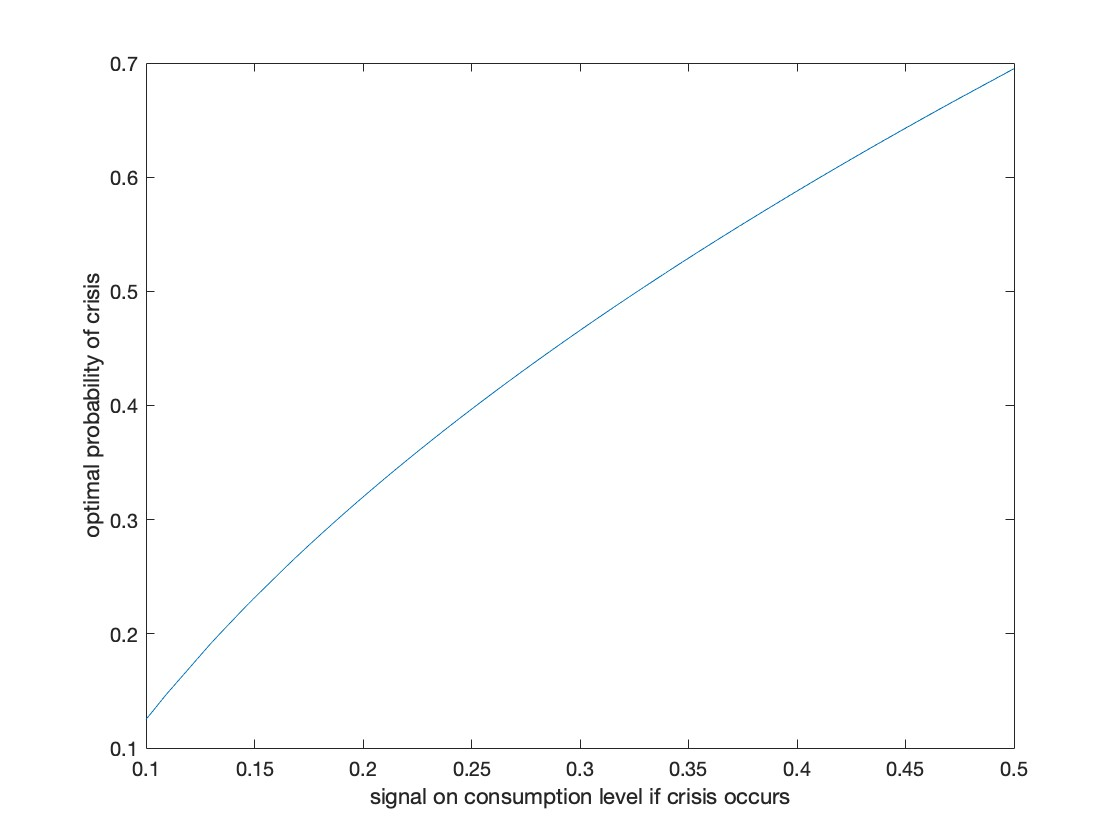
\includegraphics[width=\textwidth,height=0.4\textheight]{images/Figure1base.jpg}
\caption{Figure1}
\end{figure}

This is key in this story. How big of a risk do citizens believe to be
optimal/okay?

This model builds on Besley \& Coate (1998)'s model which selects
candidates exogenously and assumes complete information and instead
assumes imperfect information and unique signals that are randomly
provided to each voter.

\hypertarget{voters}{%
\subsection*{Voters}\label{voters}}
\addcontentsline{toc}{subsection}{Voters}

According to the median voter theorem, if preferences are single peaked
(which is implied by the uniformly distributed signals that determine
preferences and beliefs about the probability of crisis) then the median
voter will be the winning candidate in a vote, if we assume voter
sincerity (*ref).

Assume simple majority voting and that each candidate could be running
for public office, thus each voter considers each pairwise comparison
between each individual. Voters are assumed to know that candidates
could only implement their preferred policy, in this context their
individual optimal consumption point and how this maps onto their
optimal probability of crisis. Besley \& Coate (1998) voters voting
decisions are their best response given the rest of voters decisions.
Use the same assumption that candidates cannot credibly commit to any
other policy other than their own policy preference and voters know
this, which is realistic.

Besley \& Coate (1998) finds that according to the median voter result
and Condorcet Jury theorem, there is one ultimate winning candidate
which is the median voter.

\hypertarget{model-set-up-of-sustainable-consumption-in-two-country-economy-with-bargaining}{%
\section{Model set-up of sustainable consumption in two-country economy
with
bargaining}\label{model-set-up-of-sustainable-consumption-in-two-country-economy-with-bargaining}}

The impact of another country may impact the optimal level of
consumption. More realistic to consider countries' interdependent
impact, for example in IEA, especially considering that global climate
change cannot be achieved by one country acting unilaterally (ref?). As
in the global economy case, each citizen in each country receives
private signals \(\hat{\underline{c}}_k\) which determine their optimal
level of individual consumption and this maps onto their optimal
probability of crisis, because if they are signalled that climate crisis
would not reduce \(c_2\) by much, then a higher probability of this
crisis occuring is not worrisome.

First, split the global democracy into two different country populations
after each individual has received their private signals. Each
individual is divided probabilistically into country A and country B so
as to ensure random splitting. The probability of being assigned to
country A depends on two parameters (\(countryAshare\) and \(bias\)) in
addition to the cumulative density function (cdf) of each individual's
private signal. For each individual, a number is drawn between 0 and 1
and if this draw is less than or equal to the probability of country A,
then the individual is assigned to country A. If not, the individual is
assigned to country B.

\[probability_of_country A = country A share + bias(cdf_of_signal - country A share)\]

Second, the expected utilities for every possible candidate are computed
under the assumption that each citizen runs for election and promises to
implement their their ideal consumption if elected. Accordingly, each
voter considers any pairwise competition based on the expected utility
they will obtain based on their own belief about \(\tilde{c}\) as formed
due to their private signal \(\hat{\underline{c}}_k\) if the any
candidate implements their promised, preferred policy.

In addition to the fixed parameters discussed in the preceding section,
there are adjustable parameters in the two country case. Variations in
country share A can be implemented by selecting a value between 0 and
0.5, which alters the target fraction of the global democracy population
that will be probabilistically assigned to country A. Variations in bias
can be implemented by selecting a value between 0 and 0.9. This
represents the bias in country A as if the value is higher, then country
A's voters are more likely to receive higher signals and thus are more
likely to believe a higher optimal consumption level and a higher
optimal probability of crisis.

Next, find the mutual best responses Find the Nash equilibrium

Buchholz \emph{et al} (2005) compares the isolationist case against the
bargaining case with an IEA implemented between two countries to analyse
the impact of IEAs on environmental policy. Similarly, this paper
compares the global democracy of one global economy against the Nash
equilibrium solution found in the case of two countries which bargain
together according to an IEA.

\hypertarget{discussion-and-results}{%
\section{Discussion and results}\label{discussion-and-results}}

(approx 1000)

Buchholz \emph{et al} (2005) reaches an analytical result in which
voters may be incentivised to vote for less green candidates in order to
improve their own country's bargaining position when there is an IEA,
which implies that unless there is full co-operation, any bargaining
outcome is bad for environmental policy and the probability of a climate
crisis. Besley \& Coate (1998) also suggests that non-co-operation with
other countries may yield a greater expected utility than if
co-operation occurs.

Are imbalances good or bad???? Unless there is full co-operation, any
bargaining is sub-optimal

Voters in global economy vote for the median because this maximises
their expected utility.

\hypertarget{country-a-share-0-bias}{%
\subsection*{0.1 Country A share 0 Bias}\label{country-a-share-0-bias}}
\addcontentsline{toc}{subsection}{0.1 Country A share 0 Bias}

N\_A = 104, N\_B = 896 c\_average\_NE = 1.0363 prob\_crisis\_NE =0.5363

\hypertarget{country-a-share-and-0-bias}{%
\subsection*{0.5 Country A share and 0
Bias}\label{country-a-share-and-0-bias}}
\addcontentsline{toc}{subsection}{0.5 Country A share and 0 Bias}

For the base case, the share of each country is 50/50. There is no bias
introduced. Both countries receive signals that are uniformly and
normally distributed.

Size of country A is 484 and country B is 516 c\_average\_NE =1.2134
prob\_crisis\_NE = 0.7134

\hypertarget{country-a-share-0.9-bias}{%
\subsection*{0.5 Country A share 0.9
Bias}\label{country-a-share-0.9-bias}}
\addcontentsline{toc}{subsection}{0.5 Country A share 0.9 Bias}

N\_A = 523 N\_B = 477 c\_average\_NE = 1.2234 prob\_crisis\_NE =0.7234

Kemp (1976) comparative static results

\begin{center}
Table 1: Model comparison
\end{center}

\begin{longtable}[]{@{}lcc@{}}
\toprule()
& Period 1 consumption & Probability of crisis \\
\midrule()
\endhead
Global democracy & 0.9499 & 0.4499 \\
Two countries 0.1 share & 1.0363 & 0.5363 \\
Two countries 0.5 share & 1.2134 & 0.7134 \\
Two countries 0.9 bias & 1.2234 & 0.7234 \\
\bottomrule()
\end{longtable}

\hypertarget{conclusion}{%
\section{Conclusion}\label{conclusion}}

\newpage

\hypertarget{references}{%
\section*{References}\label{references}}
\addcontentsline{toc}{section}{References}

\bibliography{Tex/ref}





\end{document}
